%!TEX TS-program = xelatex

% Шаблон документа LaTeX создан в 2018 году
% Алексеем Подчезерцевым
% В качестве исходных использованы шаблоны
% 	Данилом Фёдоровых (danil@fedorovykh.ru) 
%		https://www.writelatex.com/coursera/latex/5.2.2
%	LaTeX-шаблон для русской кандидатской диссертации и её автореферата.
%		https://github.com/AndreyAkinshin/Russian-Phd-LaTeX-Dissertation-Template

\documentclass[a4paper,14pt]{article}


%%% Работа с русским языком
\usepackage[english,russian]{babel}   %% загружает пакет многоязыковой вёрстки
\usepackage{fontspec}      %% подготавливает загрузку шрифтов Open Type, True Type и др.
\defaultfontfeatures{Ligatures={TeX},Renderer=Basic}  %% свойства шрифтов по умолчанию
\setmainfont[Ligatures={TeX,Historic}]{Times New Roman} %% задаёт основной шрифт документа
\setsansfont{Comic Sans MS}                    %% задаёт шрифт без засечек
\setmonofont{Courier New}
\usepackage{indentfirst}
\frenchspacing

\renewcommand{\epsilon}{\ensuremath{\varepsilon}}
\renewcommand{\phi}{\ensuremath{\varphi}}
\renewcommand{\kappa}{\ensuremath{\varkappa}}
\renewcommand{\le}{\ensuremath{\leqslant}}
\renewcommand{\leq}{\ensuremath{\leqslant}}
\renewcommand{\ge}{\ensuremath{\geqslant}}
\renewcommand{\geq}{\ensuremath{\geqslant}}
\renewcommand{\emptyset}{\varnothing}

%%% Дополнительная работа с математикой
\usepackage{amsmath,amsfonts,amssymb,amsthm,mathtools} % AMS
\usepackage{icomma} % "Умная" запятая: $0,2$ --- число, $0, 2$ --- перечисление

%% Номера формул
%\mathtoolsset{showonlyrefs=true} % Показывать номера только у тех формул, на которые есть \eqref{} в тексте.
%\usepackage{leqno} % Нумерация формул слева	

%% Перенос знаков в формулах (по Львовскому)
\newcommand*{\hm}[1]{#1\nobreak\discretionary{}
	{\hbox{$\mathsurround=0pt #1$}}{}}

%%% Работа с картинками
\usepackage{graphicx}  % Для вставки рисунков
\graphicspath{{images/}}  % папки с картинками
\setlength\fboxsep{3pt} % Отступ рамки \fbox{} от рисунка
\setlength\fboxrule{1pt} % Толщина линий рамки \fbox{}
\usepackage{wrapfig} % Обтекание рисунков текстом

%%% Работа с таблицами
\usepackage{array,tabularx,tabulary,booktabs} % Дополнительная работа с таблицами
\usepackage{longtable}  % Длинные таблицы
\usepackage{multirow} % Слияние строк в таблице
\usepackage{float}% http://ctan.org/pkg/float

%%% Программирование
\usepackage{etoolbox} % логические операторы


%%% Страница
\usepackage{extsizes} % Возможность сделать 14-й шрифт
\usepackage{geometry} % Простой способ задавать поля
\geometry{top=20mm}
\geometry{bottom=20mm}
\geometry{left=20mm}
\geometry{right=10mm}
%
%\usepackage{fancyhdr} % Колонтитулы
% 	\pagestyle{fancy}
%\renewcommand{\headrulewidth}{0pt}  % Толщина линейки, отчеркивающей верхний колонтитул
% 	\lfoot{Нижний левый}
% 	\rfoot{Нижний правый}
% 	\rhead{Верхний правый}
% 	\chead{Верхний в центре}
% 	\lhead{Верхний левый}
%	\cfoot{Нижний в центре} % По умолчанию здесь номер страницы

\usepackage{setspace} % Интерлиньяж
\onehalfspacing % Интерлиньяж 1.5
%\doublespacing % Интерлиньяж 2
%\singlespacing % Интерлиньяж 1

\usepackage{lastpage} % Узнать, сколько всего страниц в документе.

\usepackage{soul} % Модификаторы начертания

\usepackage{hyperref}
\usepackage[usenames,dvipsnames,svgnames,table,rgb]{xcolor}
\hypersetup{				% Гиперссылки
	unicode=true,           % русские буквы в раздела PDF
	pdftitle={Заголовок},   % Заголовок
	pdfauthor={Автор},      % Автор
	pdfsubject={Тема},      % Тема
	pdfcreator={Создатель}, % Создатель
	pdfproducer={Производитель}, % Производитель
	pdfkeywords={keyword1} {key2} {key3}, % Ключевые слова
	colorlinks=true,       	% false: ссылки в рамках; true: цветные ссылки
	linkcolor=black,          % внутренние ссылки
	citecolor=black,        % на библиографию
	filecolor=magenta,      % на файлы
	urlcolor=black           % на URL
}
\makeatletter 
\def\@biblabel#1{#1. } 
\makeatother
\usepackage{cite} % Работа с библиографией
%\usepackage[superscript]{cite} % Ссылки в верхних индексах
%\usepackage[nocompress]{cite} % 
\usepackage{csquotes} % Еще инструменты для ссылок

\usepackage{multicol} % Несколько колонок

\usepackage{tikz} % Работа с графикой
\usepackage{pgfplots}
\usepackage{pgfplotstable}

% ГОСТ заголовки
\usepackage[font=small]{caption}
%\captionsetup[table]{justification=centering, labelsep = newline} % Таблицы по правобу краю
%\captionsetup[figure]{justification=centering} % Картинки по центру


\newcommand{\tablecaption}[1]{\addtocounter{table}{1}\small \begin{flushright}\tablename \ \thetable\end{flushright}%	
\begin{center}#1\end{center}}

\newcommand{\imref}[1]{рис.~\ref{#1}}

\usepackage{multirow}
\usepackage{spreadtab}
\newcolumntype{K}[1]{@{}>{\centering\arraybackslash}p{#1cm}@{}}


\usepackage{xparse}
\usepackage{fancyvrb}

\RecustomVerbatimCommand{\VerbatimInput}{VerbatimInput}
{
	fontsize=\footnotesize    
}

\usepackage{tocloft}
\renewcommand{\cftsecleader}{\cftdotfill{\cftdotsep}}
\begin{document} % конец преамбулы, начало документа
\begin{titlepage}
	\begin{center}
 		ФЕДЕРАЛЬНОЕ  ГОСУДАРСТВЕННОЕ АВТОНОМНОЕ \\
		ОБРАЗОВАТЕЛЬНОЕ УЧРЕЖДЕНИЕ ВЫСШЕГО ОБРАЗОВАНИЯ\\
		«НАЦИОНАЛЬНЫЙ ИССЛЕДОВАТЕЛЬСКИЙ УНИВЕРСИТЕТ\\
		«ВЫСШАЯ ШКОЛА ЭКОНОМИКИ»
	\end{center}
	
	\begin{center}
		\textbf{Московский институт электроники и математики}
		
		\textbf{им. А.Н.Тихонова НИУ ВШЭ}
		
		\vspace{2ex}
		
		\textbf{Департамент компьютерной инженерии}
	\end{center}
	\vspace{1ex}	
	
	\begin{center}
	\textbf{ОТЧЕТ\\
		ПО ЛАБОРАТОРНОЙ РАБОТЕ №6
	}
	\end{center}	
	\vspace{2ex}
	\begin{center}
		по дисциплине «Проектирование систем на кристалле»
	\end{center}	

	\vspace{2ex}

	\begin{flushright}
		\textbf{Выполнили:}
		
		\vspace{2ex}
		
		Студенты группы БИВ174
		
		Бригада №5
		
		\vspace{2ex}
		
		Подчезерцев Алексей Евгеньевич
		
		Солодянкин Андрей Александрович
		\vspace{2ex}
		
	\end{flushright}

	\vfill
	\begin{center}
		Москва \the\year \, г.
	\end{center}
	
\end{titlepage}
\addtocounter{page}{1}
\tableofcontents
\pagebreak
\section{Задание}

\begin{enumerate}
	\item Разработайте принципиальную схему неприоритетного шифратора, таблица истинности
	которого приведена в Таблице 3.1. Используйте логические элементы И-НЕ, ИЛИ-НЕ;
	
	\item Исследуйте работу, синтезируйте и реализуйте на FPGA плате все приведенные в данном
	разделе примеры шифраторов;
	
	\item Исследуйте работу, синтезируйте и реализуйте на FPGA плате параметрический дешифратор
	с использованием оператора сдвига (Листинг 3.14);
	
	\item Синтезируйте описанные выше параметрические шифраторы и дешифраторы с различными
	настройками профилей оптимизации и сравните параметры полученных устройств;
	Опишите, как отличаются пути прохождения сигналов и чем это обусловлено;
	
	\item Разработайте конвертор унарного кода в код Грея.
\end{enumerate}

\section{Выполнение работы}

\subsection{Неприоритетный шифратор}
 
Была разработана схема неприоритетного шифратора в базисе И-НЕ, ИЛИ-НЕ (рис.\ref{fig:z1_schema}).

$$ f_1 = \overline{\overline{x_0 | x_1 | x_2 | x_3 | x_4 | x_5 | x_6 | x_7}} $$

$$ f_2 = \overline{\overline{x_0 | x_1 | x_2 | x_3 | x_8 | x_8 | x_{10} | x_{11}}}$$

$$ f_3 = \overline{\overline{x_0 | x_1 | x_4 | x_5 | x_8 | x_9 | x_{12} | x_{13}}}$$

$$ f_4 = \overline{\overline{x_0 | x_2 | x_4 | x_6 | x_8 | x_{10} | x_{12} | x_{14}}} $$

\begin{figure}[H]
	\centering
	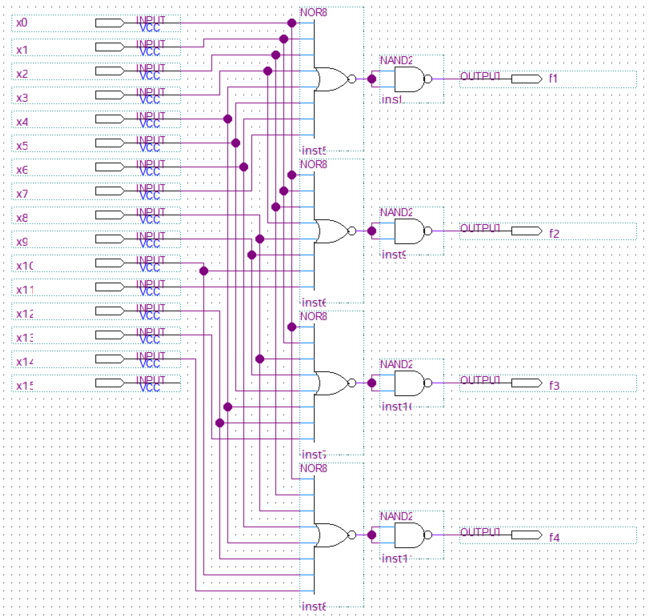
\includegraphics[width=0.9\linewidth]{imgs/z1_schema}
	\caption{Схема неприоритетного шифратора}
	\label{fig:z1_schema}
\end{figure}

\subsection{Шифраторы}

Шифратор на основе оператора непрерывного присваивания.
\VerbatimInput{../z2/b1_enc_assign.v}

Шифратор на основе оператора if.
\VerbatimInput{../z2/b2_enc_if.v}

Шифратор на основе оператора case.
\VerbatimInput{../z2/b3_enc_case.v}

Приоритетный шифратор на основе оператора if.
\VerbatimInput{../z2/b4_pri_enc_if.v}

Приоритетный шифратор на основе оператора непрерывного присваивания.
\VerbatimInput{../z2/b5_pri_enc_assign.v}

Приоритетный шифратор на основе оператора сдвиговых регистров.
\VerbatimInput{../z2/b12_anybit_enc.v}

\subsection{Дешифраторы}

\VerbatimInput{../z3/7_lab3_hdl_4bit_dec_shift/lab3.v}

\subsection{Анализ параметров оптимизации}

Было проведено тестирование параметрического шифратора и дешифратора с различными способами оптимизации схемы.

\begin{table}[H]
	\begin{center}
		\begin{flushleft}
			\tablecaption{Результаты различных вариантов оптимизации параметрического шифратора}
		\end{flushleft}
		\label{tab:encdoder}
		\begin{tabular}{|c|c|c|c|c|}
			\hline
			& slack & data delay & total delay IC & total delay cell \\ \hline
			balanced & 1.173 & 2.007      & 1.016          & 0.784            \\ \hline
			power    & 0.051 & 2.921      & 1.209          & 1.505            \\ \hline
			resource & 0.051 & 2.921      & 1.209          & 1.505            \\ \hline
			timing   & 1.025 & 1.948      & 0.921          & 0.82             \\ \hline
		\end{tabular}
	\end{center}
\end{table}

\begin{table}[H]
	\begin{center}
		\begin{flushleft}
			\tablecaption{Результаты различных вариантов оптимизации параметрического дешифратора}
		\end{flushleft}
		\label{tab:decoder}
		\begin{tabular}{|c|c|c|c|c|}
			\hline
			& slack & data delay & total delay IC & total delay cell \\ \hline
			balanced & 1.504 & 1.468      & 0.609          & 0.652            \\ \hline
			power    & 0.664 & 2.307      & 1.164          & 0.936            \\ \hline
			resource & 0.664 & 2.307      & 1.164          & 0.936            \\ \hline
			timing   & 1.648 & 1.324      & 0.583          & 0.534            \\ \hline
		\end{tabular}
	\end{center}
\end{table}

\subsection{Конвертор унарного кода в код Грея}

\VerbatimInput{../gray_case.v}

Результаты симуляции изображен на рис.\ref{fig:gray_sim}.
\begin{figure}[H]
	\centering
	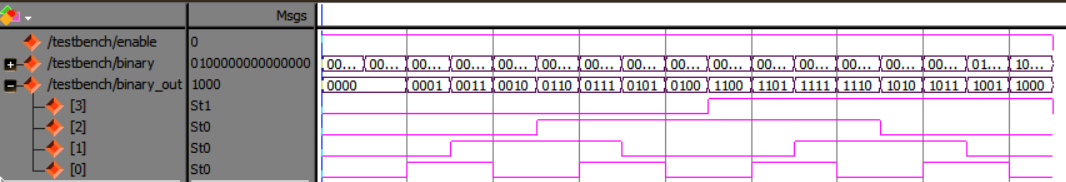
\includegraphics[width=0.9\linewidth]{imgs/gray_sim}
	\caption{Результат симуляции конвертера унарного кода в код Грея}
	\label{fig:gray_sim}
\end{figure}
 
\section{Контрольные вопросы}

\begin{enumerate}
	\item Опишите, что такое шифратор. 
	Каковы различия между приоритетным и неприоритетным шифраторами?
	
	Шифратор -- устройство, которое преобразует входной унарный код в двоичный меньшей разрядности.
	Приоритетный шифратор может обрабатывать не только унарный код, но и с несколькими логическими 1. 
	На выходе будет такой сигнал, который соответствует входному с наибольшим приоритетом.
	Неприоритетный такую работу не поддерживает.
	
	\item Опишите, как реализовать неприоритетный шифратор с помощью операторов assign,	if и case. 
	В чем их различия? 
	Какой способ лучше?
	
	Шифратор на операторе assign самый простой, однако требует аккуратности при проектировании.
	Шифратор на операторе if выглядит громоздко как и при проектировании, так и при генерации схемы.
	Шифратор на операторе case более простой с точки зрения написания кода и итоговой схемы.
	
	Однако по временным задержкам самый быстрый шифратор на операторе assign.
	
	\item Опишите, как реализовать приоритетный шифратор с помощью операторов assign и if. 
	В чем их различия? 
	Какой способ лучше?
	
	Приоритетный шифратор реализуется путем последовательной проверки каждого бита входного сигнала.
	Проверка реализуется через if или тернарный оператор и assign.
	Результат моделирования данных схем одинаковый.
	
	\item Что характеризуют такие параметры как задержка распространения ($t_{pd}$) и задержка реакции ($t_{cd}$)?
	
	Задержка распространения -- это максимальное время от начала изменения входного сигнала схемы до момента, когда	все ее выходы достигнут своих стационарных состояний.
	
	Задержка реакции -- это	минимальное время от момента, когда входной сигнал изменился, до момента, когда любой из выходов начнет менять свое значение.
	
	\item Что такое критический путь? 
	Почему следует стремиться сократить критические пути в комбинационной части цифровых схем?
	
	Критический путь -- участок схемы с наибольшей задержкой. 
	Он ограничивает скорость, с которой работает микросхема.
	
	\item Опишите предназначение дешифратора и как его реализовать на Verilog.
	Приведите несколько различных вариантов.
	
	Дешифратор выполняет обратную задачу шифратора. 
	Его основное предназначение -- выбор одного из нескольких устройств или сигнала.
	Дешифратор может быть построен на основе операторов case, сдвига, а так же непрерывного присваивания.
	
	\item Как осуществлять оптимизацию при синтезе в САПР Quartus Prime?
	
	Quartus Prime позволяет оптимизировать схему по быстродействию, энергопотреблению, по занимаемой площади кристалла, а так же сбалансированно.
	Опишите различные профили оптимизации в САПР Quartus Prime.
	
	В зависимости от выбранного режима улучшаются одни характеристики, другие же ухудшаются.
	Необходимо оптимизировать тот функционал, который критичен в конкретной ситуации.
	Кроме того, необходимо разработчику не забывать оптимизировать его решение.
	
\end{enumerate}

\section{Выводы по работе}

В ходе работы получен опыт проектирования схем в программе Quartus с помощью языка Verilog.
Полученное устройство было протестировано с помощью бенчтестов в программе Quartus Simulation Waveform editor и ModelSim.
В процессе работы были смоделированы различные шифраторы и дешифраторы, протестированы способы оптимизации схемы, а так же рассчитаны временные параметры схемы с различными способами оптимизации.
В процессе был получен опыт работы с платой DE10-Lite, на которой проверялась работоспособность полученного устройства.

\newpage 
\renewcommand{\refname}{{\normalsize Список использованных источников}} 
\centering 
\begin{thebibliography}{9} 
	\addcontentsline{toc}{section}{\refname} 
	\bibitem{Verilog} Thomas D., Moorby P. The Verilog Hardware Description Language. – Springer Science \& Business Media, 2008.
	\bibitem{citekey} Khor W. Y. et al. Evaluation of FPGA Based QSPI Flash Access Using Partial Reconfiguration //2019 7th International Conference on Smart Computing \& Communications (ICSCC). – IEEE, 2019. – С. 1-5
\end{thebibliography}

\end{document} % конец документа






